%% Working Paper -- ML4SCS, Leuphana Universitaet Lueneburg
%% Vorlage: UF_FRED_paper_style
\documentclass[11pt]{article}
\usepackage{UF_FRED_paper_style}

\onehalfspacing
\setlength{\droptitle}{-5em}

\title{ChewML: Klassifikation von Lebensmitteln anhand von Kaubewegungen aus AirPods-IMU-Daten}

\author{Jonah Karstens (4004353)\\%
    jonah.karstens@stud.leuphana.de\\[0.6em]%
    \normalsize Seminar \glqq Machine Learning for Smart and Connected Systems\grqq{} (ML4SCS)\\%
    \normalsize Modul 45005000 Vertiefungsmodul \textbullet{} Sommersemester 2026\\%
    \normalsize Prof.\ Dr.\ Burkhardt Funk, Maximilian Hannes Reinhardt\\%
    \normalsize Leuphana Universit\"at L\"uneburg}

\date{15.\,September 2026}

%% Deutsche Bezeichner erzwingen (greift auch, wenn babel auf die
%% englische Notloesung zurueckfaellt, weil ngerman.ldf fehlt)
\AtBeginDocument{%
  \renewcommand{\figurename}{Abbildung}%
  \renewcommand{\tablename}{Tabelle}%
  \renewcommand{\refname}{Literaturverzeichnis}%
  \renewcommand{\abstractname}{Kurzfassung}%
}

\begin{document}

{\setstretch{.8}
\maketitle

\begin{abstract}
\noindent Diese Arbeit untersucht, ob sich Lebensmittel anhand der Kaubewegung
klassifizieren lassen, die von den Inertialsensoren handelsüblicher AirPods Pro erfasst
wird. Über die iOS-App Sensor Logger wurden bei etwa 50\,Hz insgesamt 103 Aufnahmen einer
einzelnen Versuchsperson aufgezeichnet, verteilt auf die Klassen Apfel, Kaugummi, Skyr,
Stillsitzen sowie eine generische Klasse für sonstiges Essen. Aus nicht überlappenden
Zehn-Sekunden-Fenstern wurden 52 Merkmale aus Zeit- und Frequenzbereich extrahiert,
darunter eigens entwickelte Kaudynamik-Merkmale zu Impulsivität, Rhythmusregularität und
Kaufrequenz. Als Architektur dient ein hierarchischer Zwei-Stufen-Klassifikator: Ein Random
Forest trennt Stillsitzen von Essen, eine Support Vector Machine klassifiziert anschließend
das konkrete Lebensmittel. Ein methodischer Schwerpunkt liegt auf einer ehrlichen
Evaluation. Während die Genauigkeit innerhalb einzelner Aufnahmen 93,8\,\% beträgt, liegt
sie über Aufnahmen hinweg bei 88,7\,\%; durch Mehrheitsabstimmung über alle Fenster einer
Mahlzeit steigt sie auf 95,0\,\%. Ein Vergleich mit einem 1D-CNN auf Rohdaten zeigt, dass
Deep Learning bei dieser Datenmenge keinen Vorteil bringt. Eine Live-Webanwendung
demonstriert die Machbarkeit im Echtzeitbetrieb. Die zentrale Limitation ist die
Beschränkung auf eine Versuchsperson, weshalb die Übertragbarkeit auf andere Personen offen
bleibt.
\\
\\
\noindent
\textit{\textbf{Keywords: }%
Human Activity Recognition; Earable Computing; Inertialsensorik; Ernährungstracking; Support Vector Machine.} \\

\end{abstract}
}

% ==================================================
\section{Einleitung}
% ==================================================

Ein Ernährungstagebuch, das man einfach im Ohr trägt: Diese Idee bildet den Ausgangspunkt
der vorliegenden Arbeit. Die meisten heutigen Ansätze zum Ernährungstracking beruhen auf
manueller Eingabe in Apps oder auf dem Fotografieren von Mahlzeiten. Beide sind aufwendig,
fehleranfällig und werden im Alltag häufig nicht durchgehalten. Untersucht wird deshalb
eine passive Alternative, nämlich die Nutzung der Bewegungssensoren, die in AirPods Pro
ohnehin verbaut sind. Beim Kauen unterschiedlicher Lebensmittel entstehen charakteristische
Kieferbewegungen, die sich als Muster in den Beschleunigungs-, Gyroskop- und
Orientierungsdaten der im Ohr sitzenden Sensoren niederschlagen.

Die Erkennung von Kau- und Essaktivität lässt sich dem Forschungsfeld der Human Activity
Recognition zuordnen \citep[S.~33:1]{Bulling2014}, genauer dem noch jungen Teilgebiet des
\glqq Earable Computing\grqq, das Sensorik in Ohrhörern für die Aktivitätserkennung nutzt.
Arbeiten wie EarBit \citep{Bedri2017} haben gezeigt, dass Essenserkennung über Sensoren am
Ohr grundsätzlich möglich ist, allerdings meist mit spezialisierter Forschungshardware und
mehreren Sensormodalitäten. Der Reiz dieses Projekts liegt darin, ausschließlich die
IMU-Daten eines millionenfach verbreiteten Consumer-Geräts zu verwenden, ohne zusätzliche
Hardware, Mikrofone oder Kameras.

Die zentrale Forschungsfrage lautet: Können Kaubewegungen, die über die In-Ear-IMU-Sensoren
von AirPods Pro erfasst werden, genutzt werden, um verschiedene Lebensmittel zu
klassifizieren und Essen von Nicht-Essen zu unterscheiden? Zur Beantwortung wurden vier
Kernklassen definiert, die bewusst unterschiedliche Kaucharakteristiken abdecken: Apfel
(hart, knackig, impulsive Kaubewegungen), Kaugummi (gummiartig, schnelle gleichmäßige
Zyklen), Skyr (weich, löffelbar, langsame rhythmische Bewegung) und Stillsitzen. Im
Projektverlauf kam eine generische Klasse \glqq Essen\grqq{} hinzu, die beliebige weitere
Lebensmittel repräsentiert. Neben der Klassifikation selbst war ein zweites Ziel die
Umsetzung eines lauffähigen Gesamtsystems, das den Sensordatenstrom in Echtzeit
entgegennimmt und Mahlzeiten automatisch erkennt.

Das Projekt wurde als Einzelarbeit durchgeführt, beginnend erst in der fünften
Semesterwoche nach einem Gruppenwechsel, sodass Projektdefinition, Datenerhebung und
Pipeline in der verbleibenden Zeit von einer Person aufgebaut wurden.

% ==================================================
\section{Verwandte Arbeiten}
% ==================================================

Zur Einordnung wurden fünf Arbeiten analysiert: ein Scoping Review als Überblick sowie drei
Arbeiten zur ohrbasierten Ess- und Kauerkennung und eine Arbeit zur Texturerkennung über
ein In-Ear-Mikrofon.

Einen systematischen Überblick liefert das Scoping Review von \citet{Bell2020}, das 40
Feldstudien aus 33 Artikeln auswertet. Als Motivation nennen die Autoren die Schwächen der
klassischen Ernährungserhebung, die auf Selbstauskunft beruht und mit Erinnerungs\-ver\-zer\-run\-gen
behaftet ist, während tragbare Sensoren Essaktivität passiv erfassen \citep[S.~1]{Bell2020}.
Drei Befunde sind hier relevant. Bewegungssensoren dominieren das Feld: Ein
Beschleunigungssensor kommt in 25 der 40 Studien zum Einsatz, ein Gyroskop in 15 und ein
Mikrofon in acht, wobei die Bewegungssensoren meist am Handgelenk sitzen; eine
Inertialmesseinheit am Ohr taucht in genau einer Studie auf \citep[S.~9--10]{Bell2020}. Die
erfassten Zielgrößen sind Essgelegenheiten (37 Studien), Kauanzahl (drei) und
Hand-zu-Mund-Bewegungen (zwei); das konkrete Lebensmittel gehört nicht dazu
\citep[S.~10]{Bell2020}. Schließlich lassen zwei Studien das Gerät bei erkannter
Essbewegung direkt beim Nutzer nachfragen, ein Vorgehen, dessen weitere Erprobung die
Autoren empfehlen \citep[S.~9 und S.~11]{Bell2020}.

Die Studie EarBit \citep{Bedri2017} untersucht die Erkennung von Essepisoden mit am Kopf
getragenen Sensoren und nutzt Kauen als Stellvertreter für Essen. Verglichen wurden
optische, inertiale und akustische Sensorik; als beste Variante erwies sich ein
Inertialsensor hinter dem Ohr, ergänzt um einen zweiten im Nacken, der grobe
Körperbewegungen herausfiltert \citep[S.~3 und S.~11]{Bedri2017}. Im unkontrollierten
Alltagseinsatz mit zehn Teilnehmenden und 45 Stunden Aufzeichnung erkannte EarBit Kauen im
Sekundentakt mit einer Genauigkeit von 93\,\% bei einem F1-Wert von 80,1\,\%; zu
Essepisoden aggregiert wurden 15 von 16 Mahlzeiten erkannt \citep[S.~3 und S.~16]{Bedri2017}.

Der Fragestellung dieser Arbeit am nächsten kommt die Studie von
\citet{Papapanagiotou2021}, die aus dem Kaugeräusch eines In-Ear-Mikrofons auf
Eigenschaften des Lebensmittels selbst schließt. Erkannt werden drei sensorische
Texturattribute, nämlich Knusprigkeit, Feuchtigkeit und Zähigkeit, jeweils über eine eigene
binäre Support Vector Machine \citep[S.~1 und S.~3]{Papapanagiotou2021}. Der Datensatz
umfasst neun Probanden und neun Lebensmittel. Die Knusprigkeit erweist sich mit einer
gewichteten Genauigkeit von mindestens 0,90 als zuverlässigstes Attribut
\citep[S.~10]{Papapanagiotou2021}, während Feuchtigkeit und Zähigkeit deutlich schlechter
abschneiden \citep[S.~8]{Papapanagiotou2021}.

IMChew \citep{Ketmalasiri2024} untersucht, wie sich Kauaktivität und Kauanzahl allein aus
den Inertialsensoren von Ohrhörern bestimmen lassen, und grenzt mikrofonbasierte Systeme
bewusst ab, da diese im Alltag als aufdringlich gelten, während Inertialsensoren in
handelsüblichen Ohrhörern bereits serienmäßig verbaut sind \citep[S.~29]{Ketmalasiri2024}.
Erhoben wurden Daten von acht Probanden mit der Forschungsplattform eSense bei 60\,Hz
\citep[S.~31]{Ketmalasiri2024}. Aus Drei-Sekunden-Fenstern werden 96 Merkmale extrahiert
\citep[S.~30--31]{Ketmalasiri2024}; unter Leave-One-Subject-Out erreicht ein Random Forest
pro Fenster 0,86, aggregiert auf Zehn-Sekunden-Episoden 0,91 \citep[S.~32]{Ketmalasiri2024}.

Die jüngste Arbeit, CHOMP \citep{Hummel2026}, stellt das erste System zur Erkennung der
Kauseite mit Ohrhörern vor; die Motivation ist medizinisch, da eine einseitige Kaupräferenz
als Risikofaktor für kraniomandibuläre Dysfunktionen gilt \citep[S.~1]{Hummel2026}. Zum
Einsatz kommen zwei Geräte der Plattform OpenEarable 2.0 mit fünf Sensormodalitäten. Die
stärkste Einzelmodalität sind die Mikrofone mit einem medianen F1-Wert von 94,5\,\% unter
Leave-One-Food-Out und 92,6\,\% unter Leave-One-Subject-Out; die IMU liegt mit 84,8
beziehungsweise 84,5\,\% im Mittel um 8,9 Prozentpunkte darunter
\citep[S.~17]{Hummel2026}.

Aus diesen Arbeiten ergibt sich eine Forschungslücke. Die Machbarkeit der Essenserkennung
am Ohr ist belegt, wobei sich bei EarBit gerade ein Inertialsensor gegenüber optischer und
akustischer Sensorik durchsetzte \citep[S.~3]{Bedri2017}. Der Kaurhythmus ist
charakterisiert: IMChew sucht die dominante Kaufrequenz zwischen 0,5 und 2,5\,Hz
\citep[S.~31]{Ketmalasiri2024}, CHOMP filtert die IMU-Kanäle mit einem Bandpass von 0,1 bis
6,0\,Hz und begründet dies damit, dass der Kaurhythmus typischerweise unter 3\,Hz liegt
\citep[S.~10]{Hummel2026}. Und feingranulare Eigenschaften des Kauens sind erkennbar, da
CHOMP die Kauseite allein aus IMU-Daten mit einem medianen F1-Wert von 84,5\,\% über
unbekannte Probanden unterscheidet \citep[S.~17]{Hummel2026}. Das konkrete Lebensmittel ist
dagegen in keiner der betrachteten Arbeiten Zielgröße; unter 40 ausgewerteten Feldstudien
nutzt genau eine eine ohrgetragene IMU, und keine erfasst das Lebensmittel
\citep[S.~9--10]{Bell2020}. Hinzu kommt, dass sämtliche betrachteten Systeme auf
Forschungshardware beruhen. IMChew nennt die AirPods zwar ausdrücklich als Beispiel für
Ohrhörer mit serienmäßiger IMU \citep[S.~29]{Ketmalasiri2024}, erhebt seine Daten aber
nicht damit.

An diese Arbeiten knüpft das Projekt in drei Punkten an, die dort nicht vorkommen: die
Unterscheidung dreier bewusst sehr unterschiedlicher Lebensmittel anhand ihrer
Kaubewegung, die Verwendung eines unveränderten Massenmarktprodukts statt
Forschungshardware und die Umsetzung als Echtzeitsystem bis zur Erkennung einer Mahlzeit.
Zwei Entscheidungen sind aus der Literatur übernommen: der Frequenzbereich der
Kaumerkmale, hier mit 0,5 bis 4\,Hz an der Obergrenze etwas weiter gefasst, sowie die
Validierung nach dem Prinzip des Leave-One-Subject-Out, das hier mangels weiterer Probanden
auf Aufnahmen statt Probanden angewandt wird. Die Abkürzung LOSO steht im Folgenden daher
für Leave-One-Session-Out.

% ==================================================
\section{Daten und Methodik}
% ==================================================

\subsection{Datenerhebung}

Für die Datenerhebung wurden AirPods Pro in Verbindung mit der iOS-App Sensor Logger
verwendet, die die Motion-Daten über das iPhone ausliest und als CSV-Dateien exportiert.
Aufgezeichnet wurden mit einer Abtastrate von etwa 50\,Hz die Beschleunigung der Ohrhörer,
der Gravitationsvektor, die Rotationsraten des Gyroskops sowie die Euler-Winkel. Jede
Aufnahme enthält genau eine Aktivität; die Zuordnung zur Klasse erfolgt über eine
Namenskonvention, sodass neue Aufnahmen ohne Codeänderung ergänzt werden können.

Die Erhebung erfolgte iterativ über den gesamten Projektzeitraum, beginnend mit einem
Minimaldatensatz von zwölf Aufnahmen und wachsend über 24, 72, 78 und 89 auf final 103
Aufnahmen: 27 Apfel, 28 Kaugummi, 25 Skyr, 19 Still sowie vier Aufnahmen der generischen
Klasse (reale Mahlzeiten wie Chili con Carne oder Overnight Oats). Die letzte
Erhebungsrunde diente gezielt dem Klassenausgleich, bis alle drei Speiseklassen mit 308,
312 und 343 Zeitfenstern annähernd gleich stark vertreten waren. Die Aufnahmen entstanden
über mehrere Monate zu unterschiedlichen Tageszeiten, wobei die AirPods vor jeder Aufnahme
neu eingesetzt wurden, sodass sich Sitzposition und Sensorlage zwischen den Aufnahmen
unterscheiden. Abbildung~\ref{fig:daten} zeigt die Verteilung.

\begin{figure}[H]
    \centering
    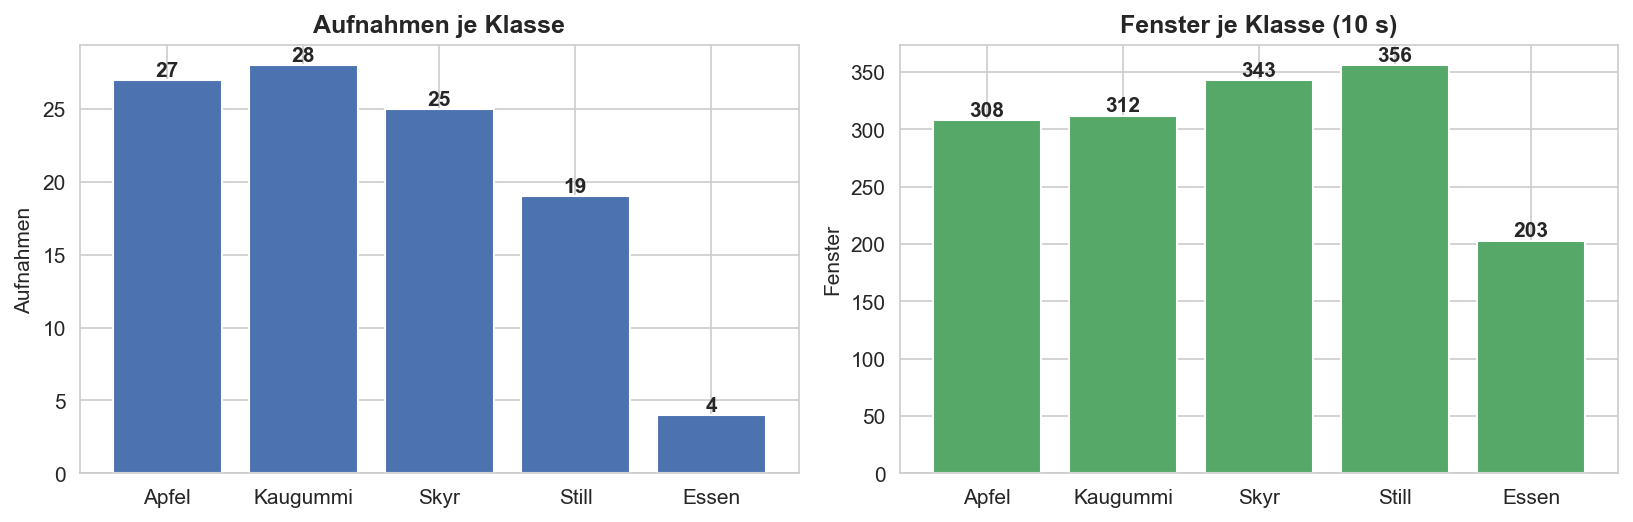
\includegraphics[width=.62\textwidth]{figures/final_daten.png}
    \caption{Finaler Datensatz: 103 Aufnahmen einer Versuchsperson, Verteilung pro Klasse.}
    \label{fig:daten}
\end{figure}


Bereits die visuelle Inspektion der Rohsignale zeigt deutliche Klassenunterschiede
(Abbildung~\ref{fig:signal}): Stillsitzen erzeugt ein nahezu flaches Magnitudensignal mit
sehr geringer Varianz, während alle Essklassen rhythmische Oszillationen mit
klassenspezifischer Amplitude und Frequenz aufweisen.

\begin{figure}[H]
    \centering
    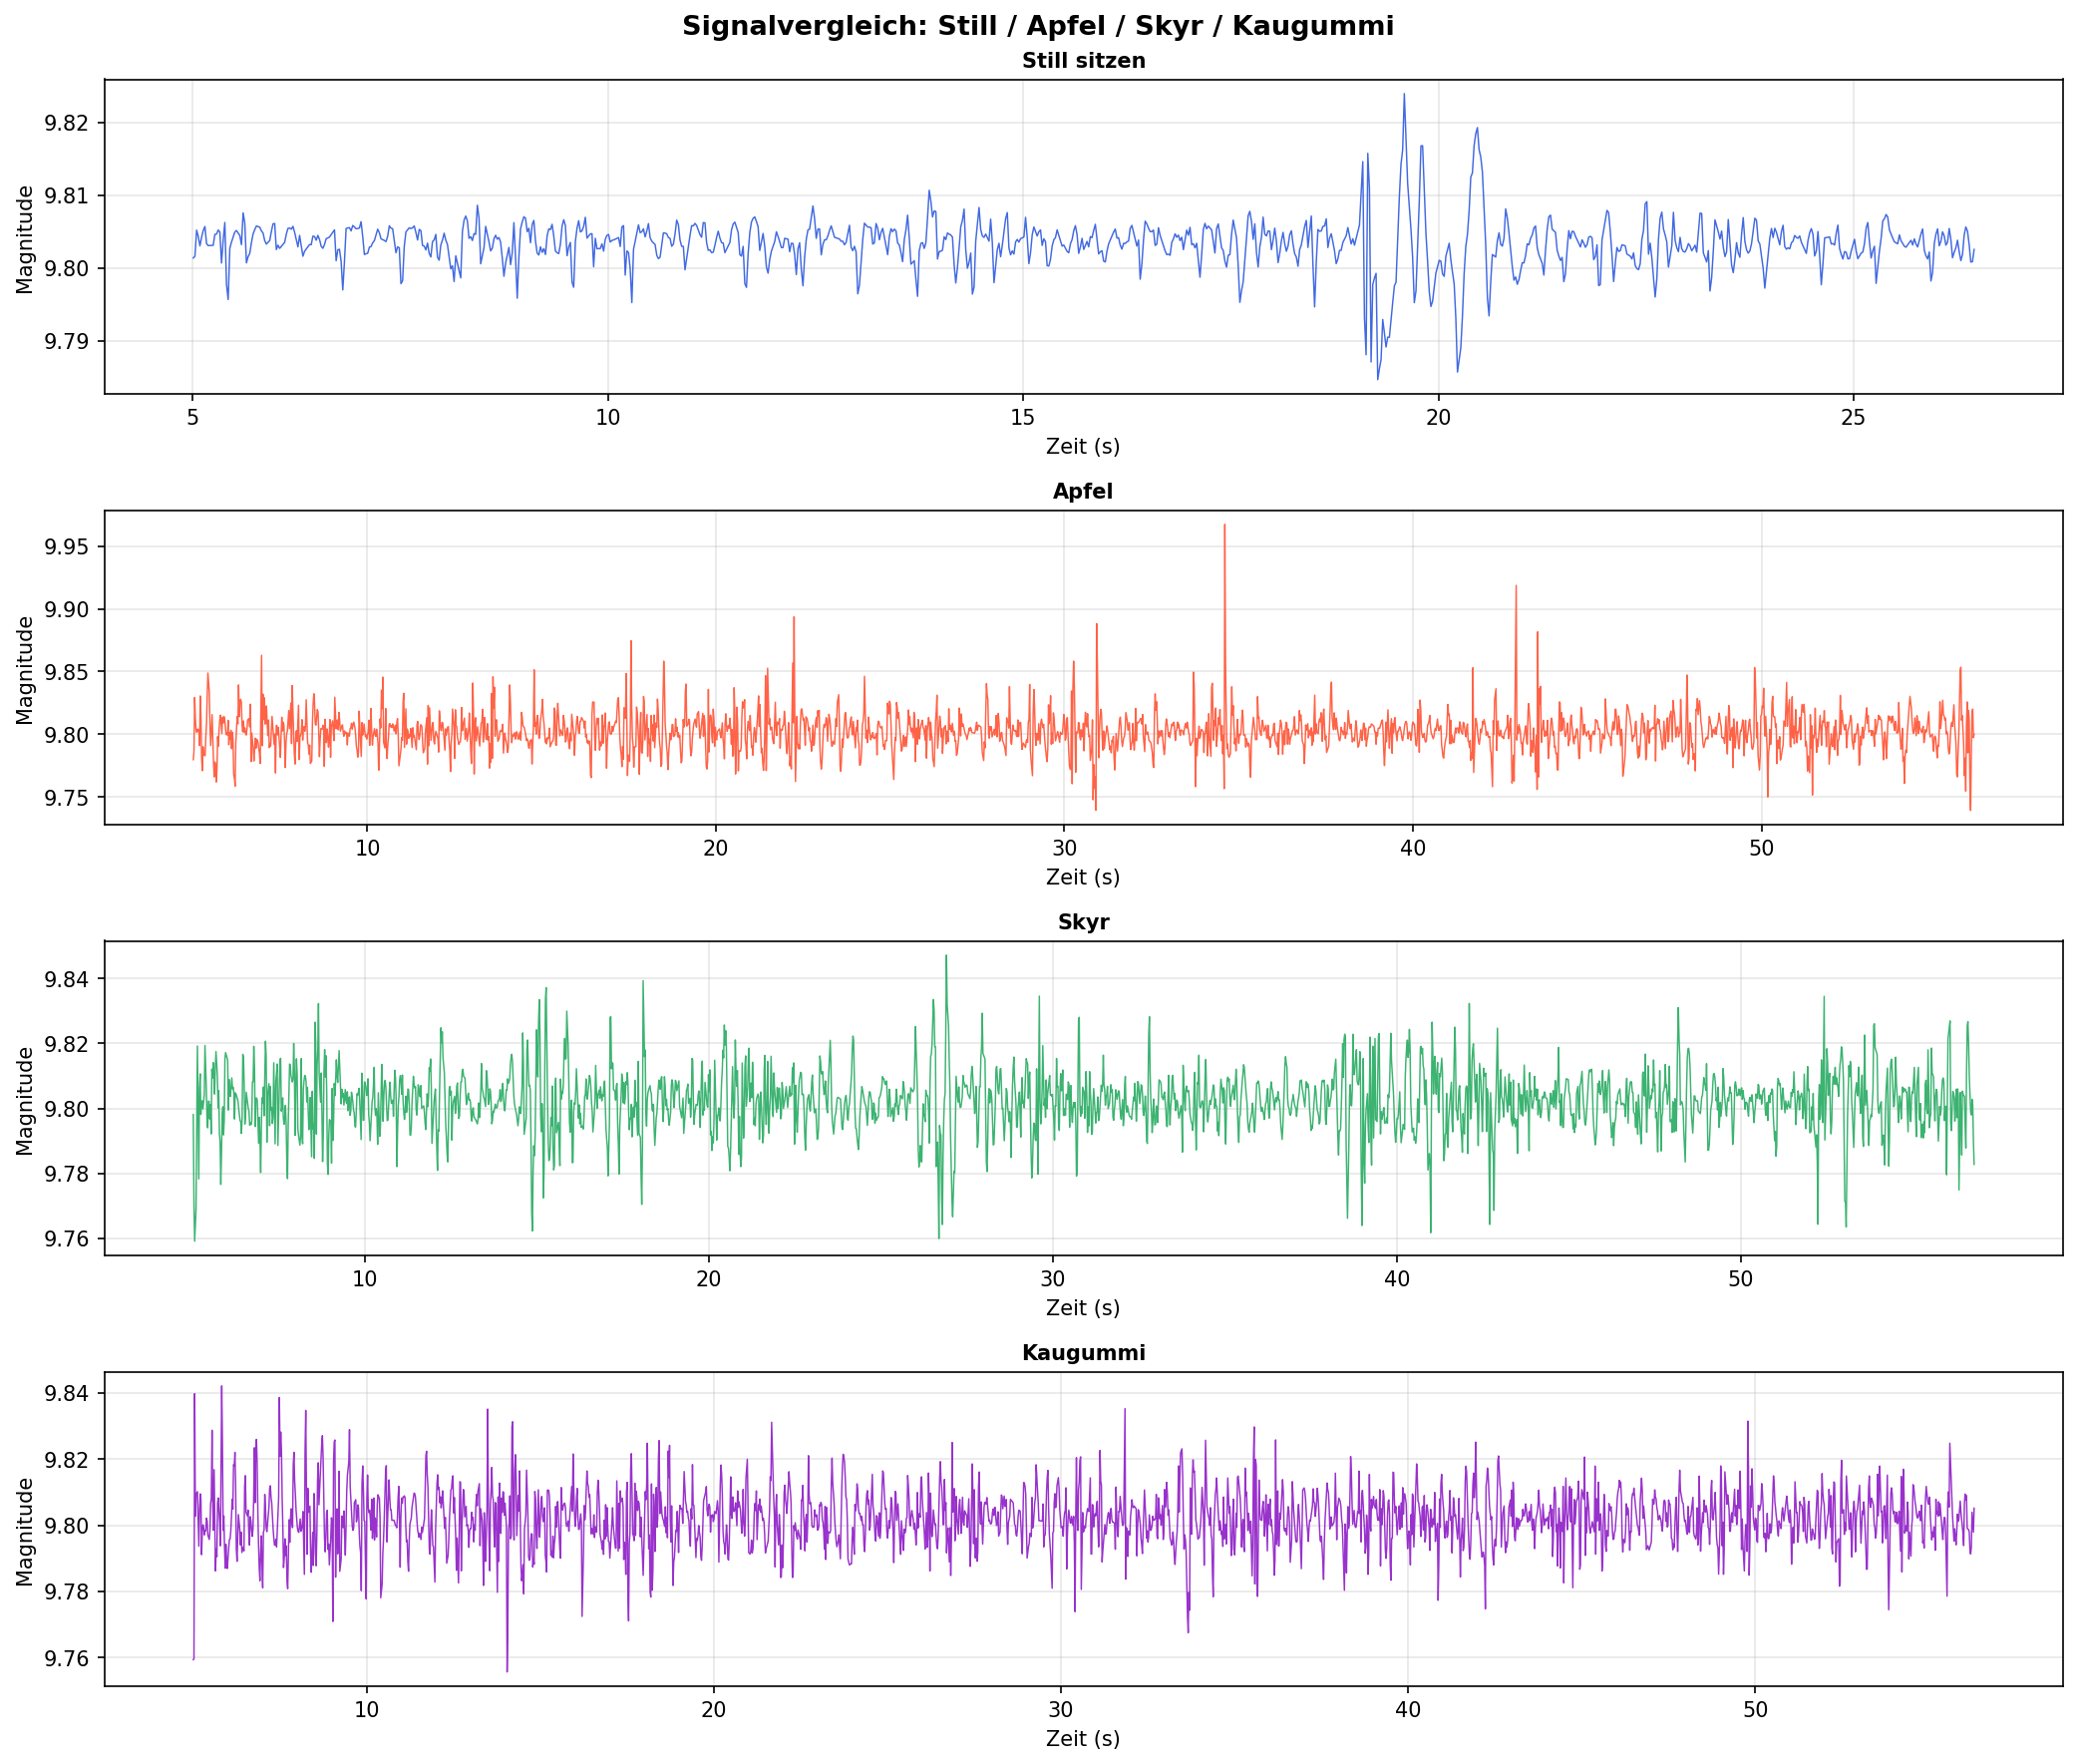
\includegraphics[width=.86\textwidth]{figures/alle_klassen_signal.png}
    \caption{Magnitudensignal über die Zeit für eine repräsentative Aufnahme pro Klasse.}
    \label{fig:signal}
\end{figure}

Zwei Erkenntnisse prägten den weiteren Verlauf. Erstens erwies sich die Datenqualität als
kritischer Faktor, da einzelne Aufnahmen mehrsekündige Kopfbewegungsphasen enthalten, die
physikalisch nichts mit dem Essen zu tun haben, aber die Merkmalsstatistiken verfälschen.
Zweitens stammen sämtliche Aufnahmen von einer einzigen Versuchsperson; die geplante
Erhebung weiterer Probanden ließ sich im Projektzeitraum nicht realisieren, und eine Suche
nach öffentlich verfügbaren Datensätzen mit vergleichbaren Kauaufnahmen blieb erfolglos.

\subsection{Vorverarbeitung}

Von jeder Aufnahme wurden die ersten und letzten zwei Sekunden entfernt, um Artefakte beim
Starten und Stoppen auszuschließen. Auf eine Subtraktion des Gravitationsanteils wurde
bewusst verzichtet, da die beiden Größen in unterschiedlichen Einheiten vorliegen: Die
Beschleunigungsachsen werden in Vielfachen der Erdbeschleunigung ausgegeben, der
Gravitationsvektor dagegen in m/s$^2$ (\citeauthor{Choi}, o.\,J.). Hinzu kommt, dass die
Beschleunigungswerte aus der Sensorfusion des Betriebssystems stammen und die
Erdbeschleunigung bereits nicht mehr enthalten; ihr Betrag liegt im Median deutlich unter
0,1\,g, während der Gravitationsvektor durchgehend den Betrag 9,807\,m/s$^2$ aufweist. Ein
früher Versuch, ihn dennoch abzuziehen, bestätigte das: Die Magnitude lag anschließend für
jede Klasse bei etwa 9,81, die Signale wurden flach und die Genauigkeit fiel auf rund
70\,\%. Aus den unverändert übernommenen Achsen wurde ein skalares Magnitudensignal
gebildet, das die Gesamtintensität der Kopf- und Kieferbewegung unabhängig von der
Sensororientierung erfasst und die Grundlage der meisten frequenzbasierten Merkmale bildet.

Zwei klassische Filteransätze wurden untersucht. Ein Butterworth-Tiefpassfilter vierter
Ordnung, dessen kennzeichnende Eigenschaft ein im Durchlassbereich gleichmäßiger
Frequenzgang ist \citep[S.~536]{Butterworth1930}, wurde nullphasig mit Grenzfrequenzen von
1, 2, 4 und 6\,Hz angewendet. Für sich genommen hilft er deutlich, da die Genauigkeit von
85,0\,\% ohne Filterung auf 93,3\,\% bei 4\,Hz steigt. In Kombination mit der unten
beschriebenen Movement-Segment-Exclusion kehrt sich das Bild jedoch um: Diese erreicht
allein 98,3\,\%, zusammen mit dem Tiefpass nur noch 91,7\,\%. Beide Schritte setzen an
derselben Störung an, und die Glättung verschlechtert die Grundlage, auf der die Movement
Exclusion ihren Schwellwert bildet. In der finalen Pipeline wird daher kein Tiefpass
eingesetzt. Ein Hampel-Filter, der jeden Messwert mit dem gleitenden Median seiner Umgebung
vergleicht und ihn ersetzt, wenn er weiter als ein Vielfaches der über die mediane absolute
Abweichung geschätzten Streuung entfernt liegt \citep[S.~2]{Pearson2016}, entfernte bei
3\,$\sigma$ fälschlich echte Kauspitzen und ließ die Genauigkeit bei 5\,$\sigma$
unverändert. Beide Experimente führten zum selben Schluss: Weder hochfrequentes Rauschen
noch isolierte Ausreißer verursachen die Fehlklassifikationen, sondern anhaltende
Kopfbewegungsphasen.

Daraus entstand ein eigener Ansatz, der zusammenhängende Bewegungsphasen ausschließt statt
einzelner Datenpunkte. Für jedes auszuwertende Zeitfenster wird ein adaptiver Schwellwert
als $\max(0{,}02\,\mathrm{g},\ 5 \times \mathrm{Median\ der\ Fenster\text{-}Magnitude})$
berechnet. Er skaliert damit automatisch mit dem Grundrauschen des Fensters, ohne
Klassenlabels zu benötigen, und liefert Werte, die der Domänenintuition entsprechen
(typisch je Klasse: Still 0,020\,g, Skyr 0,060\,g, Apfel 0,095\,g). Ein gleitendes Maximum
über eine Sekunde sorgt dafür, dass ganze kontaminierte Abschnitte entfernt werden
(Abbildung~\ref{fig:me}). Auf dem damaligen Datensatz von 24 Aufnahmen hob dieser Schritt
die Genauigkeit von 87,5\,\% auf 100\,\% und war der bis dahin größte Einzeleffekt. Später
zeigte die Fehleranalyse jedoch, dass er auch die impulsiven Crunch-Spitzen des Apfels
entfernt, also genau jene Signalanteile, die den harten Apfel von weichem Essen
unterscheiden. Die finale Architektur verwendet ihn daher hybrid: Stufe~1 nutzt ihn immer,
Stufe~2 arbeitet ohne ihn.

\begin{figure}[H]
    \centering
    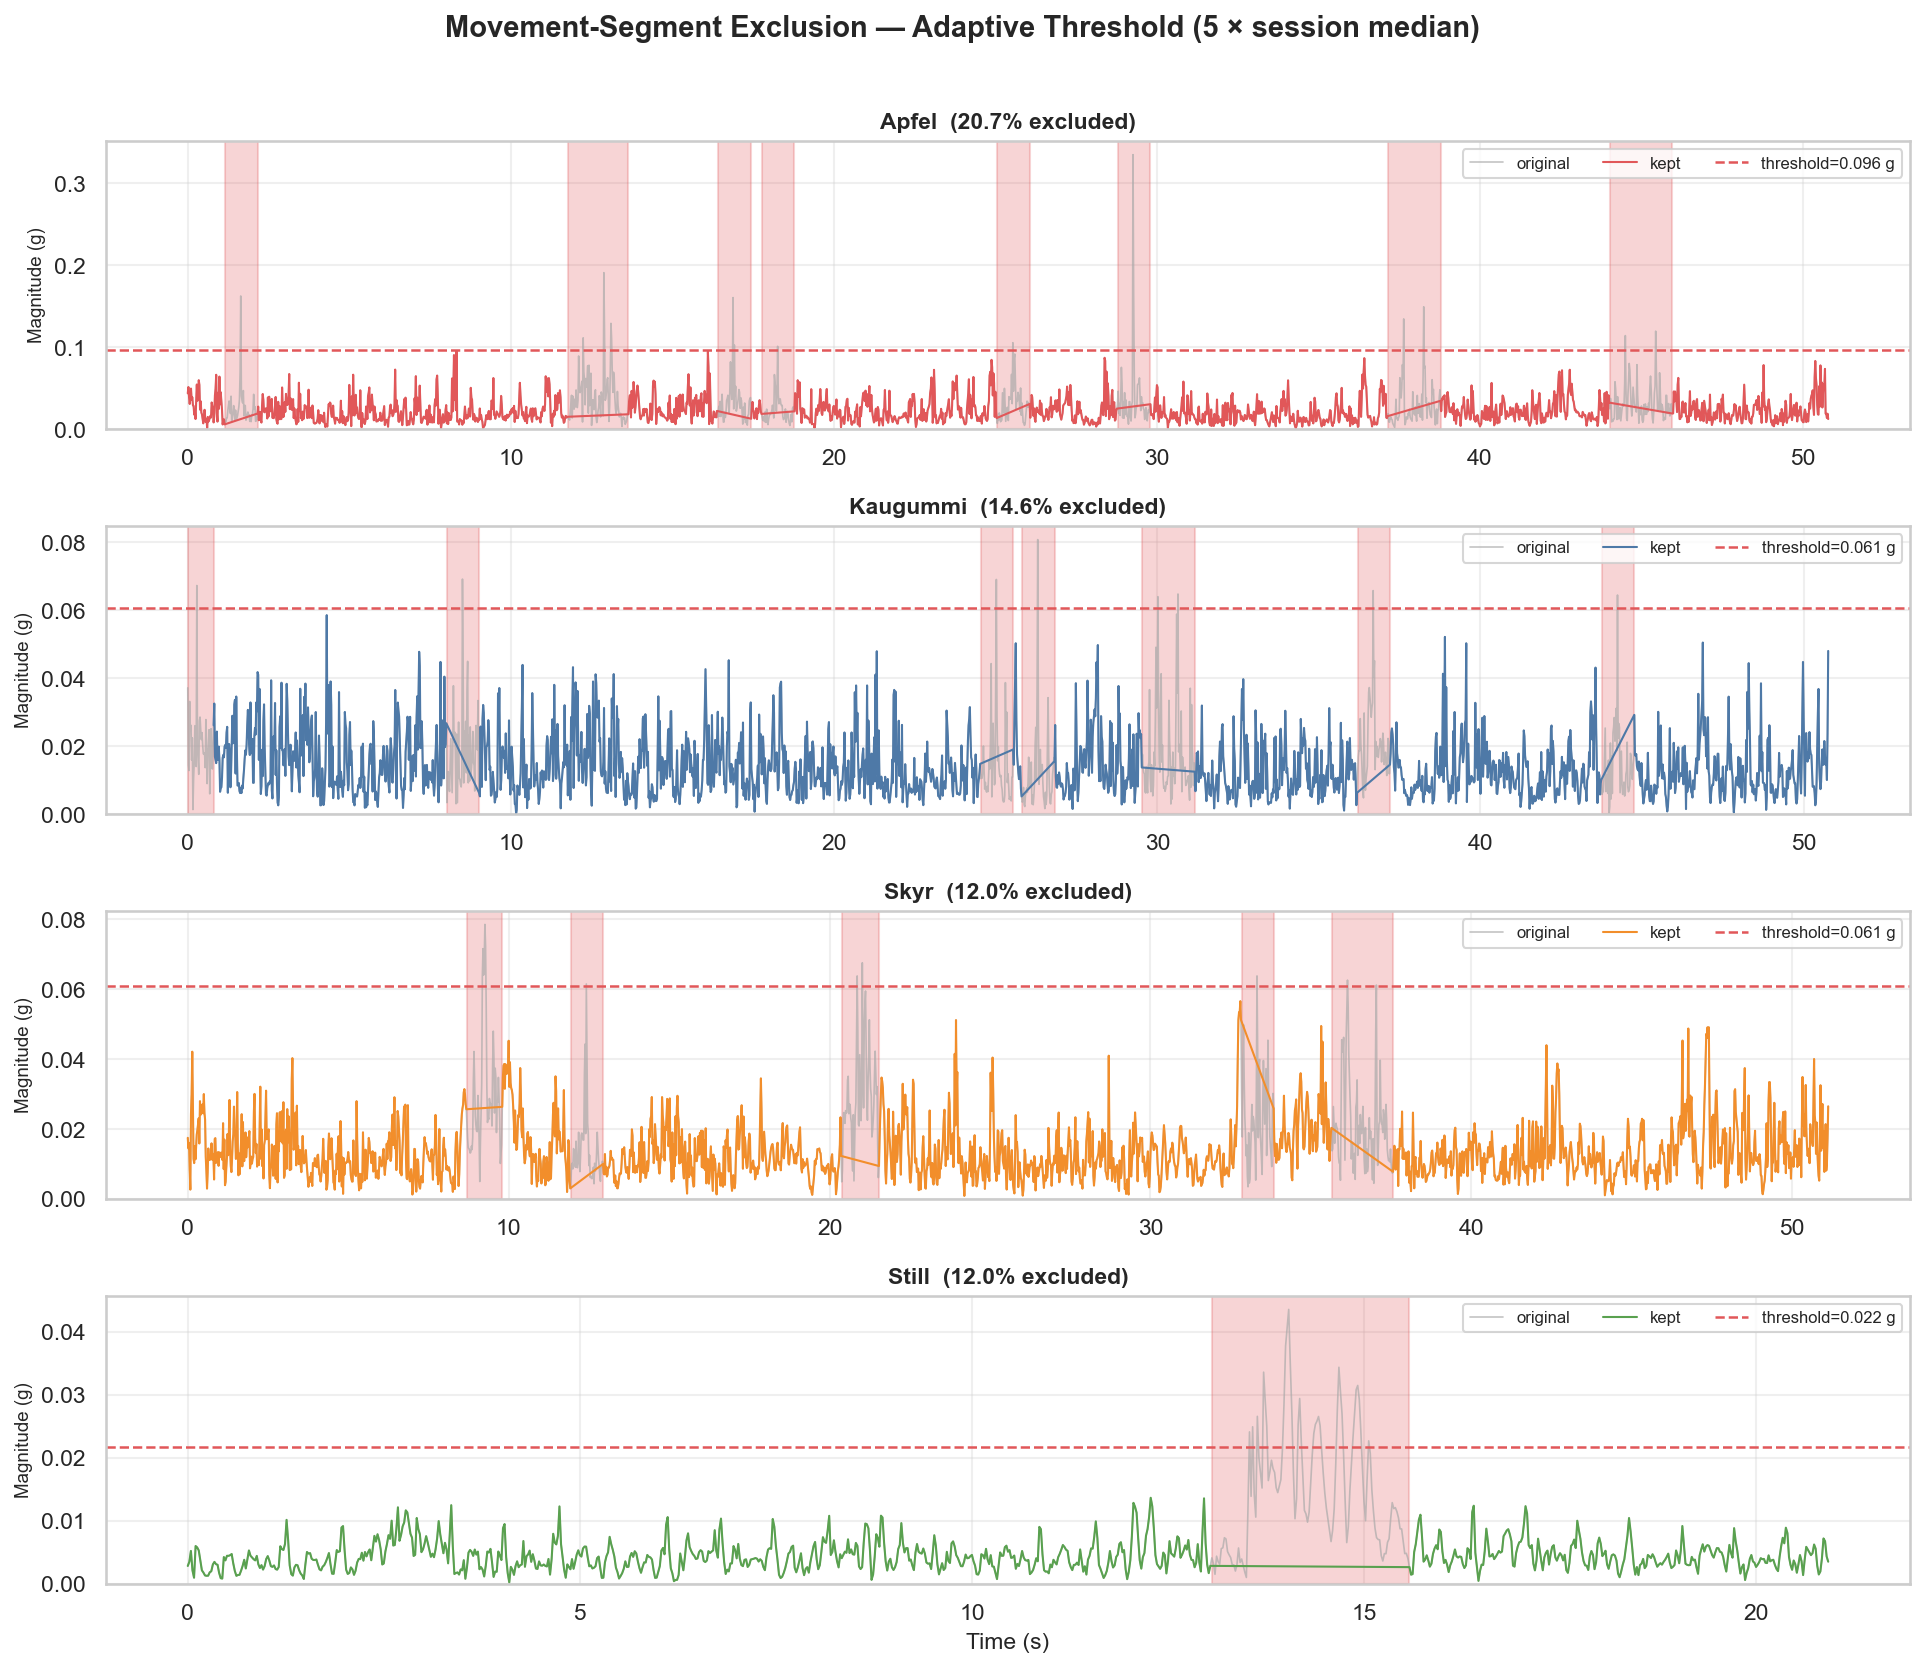
\includegraphics[width=.86\textwidth]{figures/movement_exclusion.png}
    \caption{Movement-Segment-Exclusion mit adaptivem Schwellwert (gestrichelt) für je eine
    Aufnahme pro Klasse. Rot schattierte Bereiche werden ausgeschlossen. Die Grafik stammt
    aus der frühen Analysephase mit sessionweisem Median; die finale Pipeline bildet den
    Median pro Zehn-Sekunden-Fenster.}
    \label{fig:me}
\end{figure}

Die Aufnahmen wurden in nicht überlappende Zeitfenster von einheitlich zehn Sekunden
unterteilt, sodass Offline-Evaluation und Echtzeitbetrieb dieselbe Segmentierung verwenden.
Kürzere Fenster kosten etwas Genauigkeit, sind für den Livebetrieb aber nötig, weil die
Fensterlänge unmittelbar bestimmt, wie lange ein Erkennungssystem auf sein erstes Ergebnis
warten muss \citep[S.~33:10]{Bulling2014}. Ein Experiment mit überlappenden Fenstern zeigte
das Gegenteil des Erhofften: Je stärker die Überlappung, desto schlechter die
sessionübergreifende Genauigkeit, die trotz einer auf 2409 aufgeblähten Fensteranzahl von
76\,\% auf etwa 71\,\% fiel. Überlappende Fenster derselben Aufnahme sind stark korreliert
und erhöhen die scheinbare Datenmenge, ohne neue Information beizutragen.

\subsection{Merkmale und Merkmalsauswahl}

Pro Zeitfenster wurden zunächst 36 Basismerkmale aus drei Domänen extrahiert: aus dem
Zeitbereich Mittelwert, Standardabweichung und Maximum der Beschleunigungsachsen, der
Magnitude und der Gyroskopachsen sowie der Anteil sehr ruhiger Datenpunkte und die Anzahl
der Bewegungsereignisse; aus den Euler-Winkeln Mittelwert, Standardabweichung und
Wertebereich; aus dem Frequenzbereich auf Basis der Welch-Leistungsspektraldichte die
dominante Kaufrequenz im Band von 0,5 bis 4\,Hz, die Bandleistung, die Gesamtleistung sowie
deren Verhältnis als Maß der Rhythmizität.

Da diese statistischen Merkmale die feinen Unterschiede zwischen den Esstexturen nur
unvollständig erfassten, wurden 16 weitere Merkmale entworfen, jeweils ausgehend von einer
physikalischen Annahme. Die erste betrifft den Apfel: Ein harter Biss sollte kurze,
kräftige Impulse auf ruhigem Grund erzeugen. Umgesetzt wurde das über Wölbung und Schiefe
der Amplitudenverteilung, den Crest-Faktor sowie den Jerk, also die zeitliche Ableitung der
Beschleunigung. Bestätigt hat sich davon vor allem der Jerk, dessen Mittelwert im finalen
Modell mit deutlichem Abstand das wichtigste Merkmal ist und dessen Streuung auf Rang vier
folgt, während von den Formmaßen nur die Wölbung erhalten bleibt. Die zweite Annahme
betrifft das Kaugummi, bei dem derselbe Bewegungsablauf wiederholt wird und das Signal
daher ausgeprägt periodisch sein sollte. Umgesetzt wurde das über die Autokorrelation,
deren höchstes Nebenmaximum im Kauband die Wiederholgenauigkeit angibt, sowie über die
Anzahl erkannter Kauspitzen pro Sekunde und die Streuung ihrer Abstände. Diese Annahme hat
sich bestätigt, da alle vier rhythmusbezogenen Merkmale erhalten bleiben und zwei davon
unter den ersten zehn stehen. Der Merkmalssatz umfasst damit 52 Werte pro Zeitfenster.

Die Merkmalsselektion erwies sich als eines der schwierigsten Teilprobleme und wurde für
beide Stufen getrennt durchgeführt. Für Stufe~1 wählte eine rekursive
Merkmalseliminierung, die wiederholt ein Modell trainiert und jeweils das schwächste
Merkmal entfernt \citep[S.~394]{Guyon2002}, in einem frühen Versuch nur fünf Merkmale aus.
Dieser Satz erfasste im Wesentlichen die Bewegungsstärke und wertete dadurch jede
Kopfbewegung als Essen; er wurde durch 14 Merkmale ersetzt, die zusätzlich den Kaurhythmus
einbeziehen. Für Stufe~2 verschlechterte dasselbe Verfahren die Genauigkeit, da alle drei
Klassen Kaubewegungen sind und viele Merkmale überlappende Information tragen. Verwendet
wurde daher eine gruppenbewusste Permutation Importance, bei der die Werte eines Merkmals
zufällig durchmischt werden und gemessen wird, wie stark die Genauigkeit fällt. Dass die
Aufnahmen als Gruppen behandelt werden, sorgt dafür, dass die Bewertung die Generalisierung
über Aufnahmen hinweg abbildet. Von den 52 Merkmalen leisten 39 einen positiven Beitrag
(Abbildung~\ref{fig:fs}); die entfernten sind überwiegend absolute Lage- und
Orientierungswerte, die nicht das Kauen, sondern die zufällige Kopfhaltung während einer
Aufnahme beschreiben.

\begin{figure}[H]
    \centering
    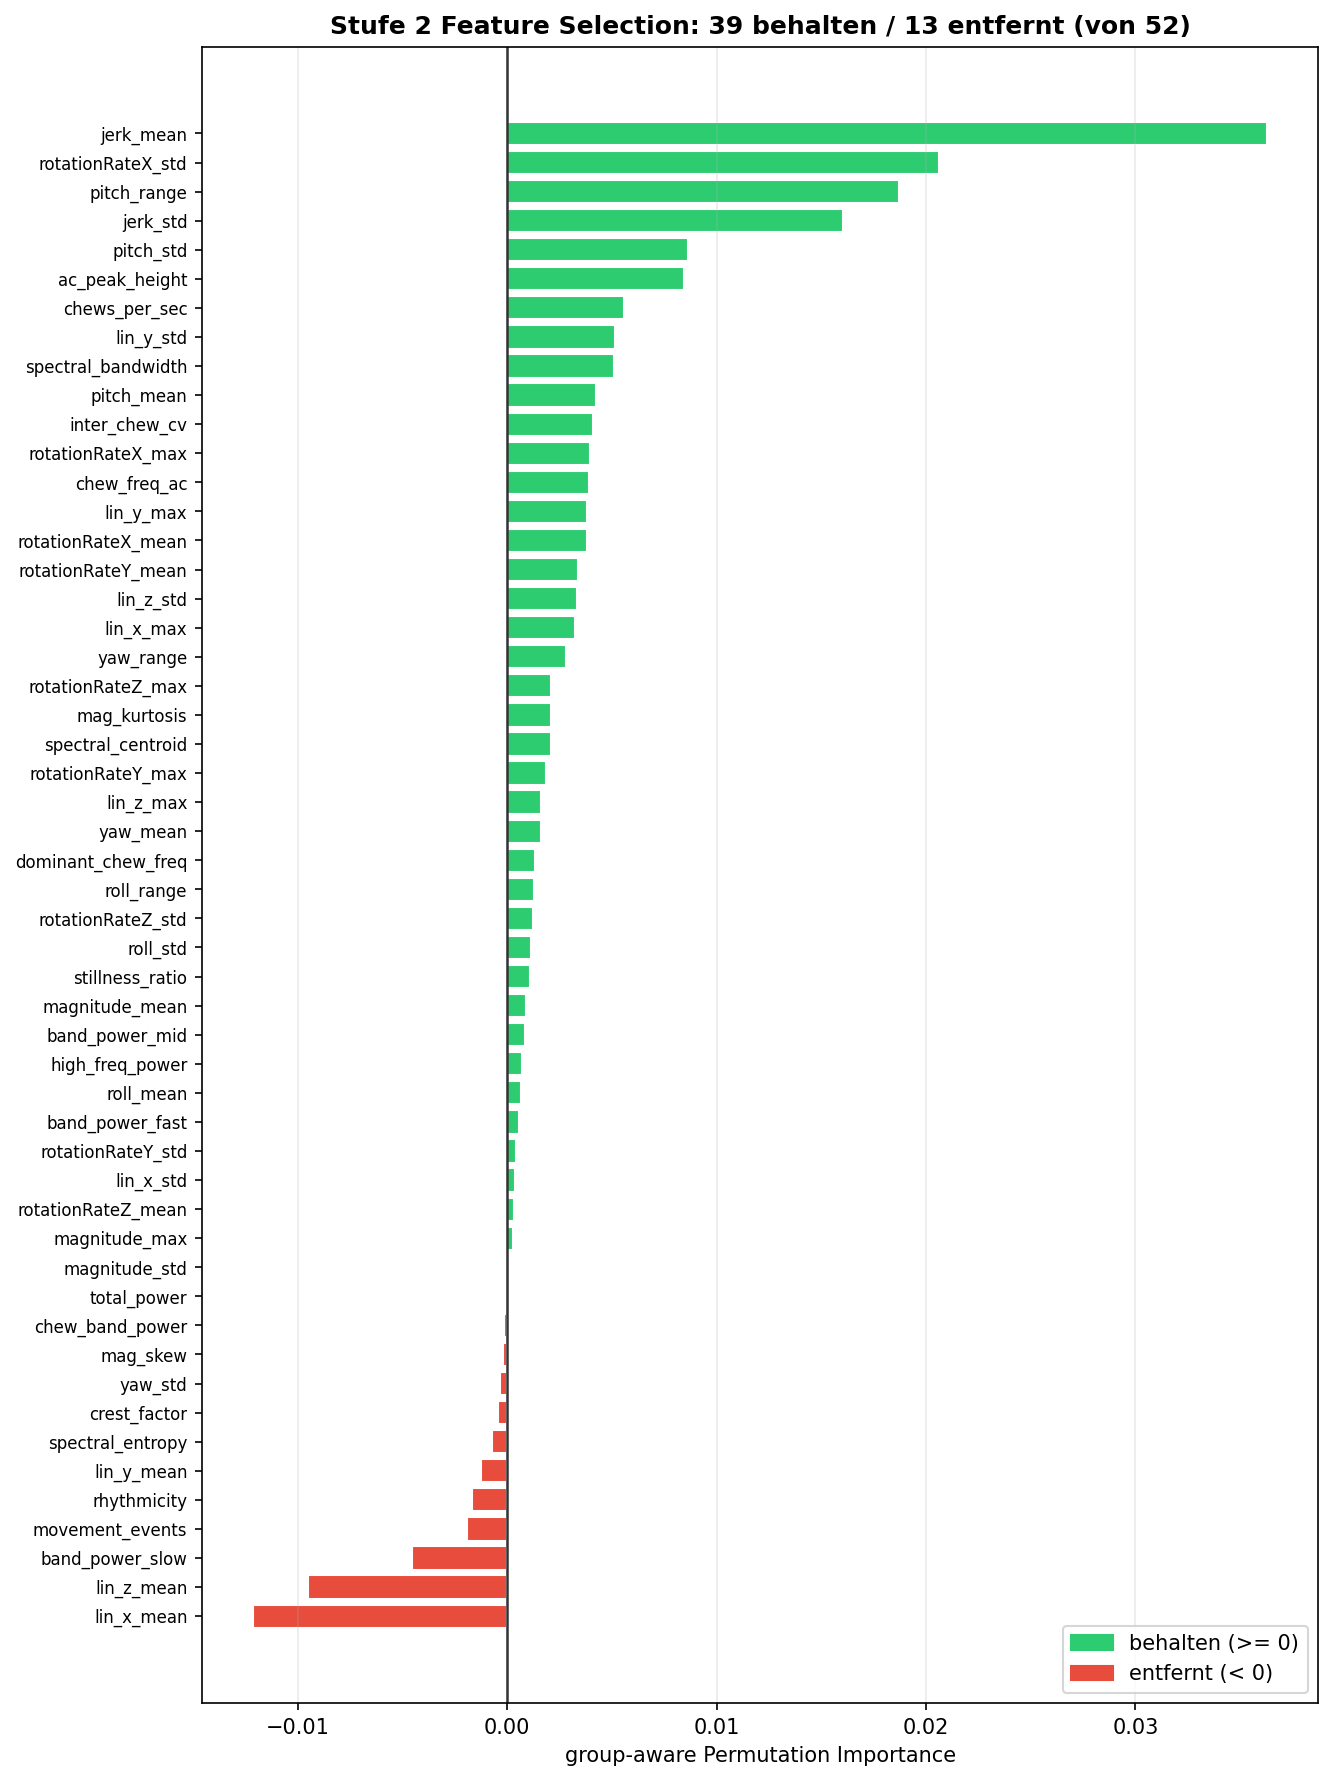
\includegraphics[width=.60\textwidth]{figures/nb14_feature_selection_s2.png}
    \caption{Gruppenbewusste Permutation Importance aller 52 Merkmale für Stufe~2.
    Grün: behalten, rot: entfernt.}
    \label{fig:fs}
\end{figure}

\subsection{Modellarchitektur und Evaluationsdesign}

Anstelle eines flachen Klassifikators wurde das Problem in zwei Teilprobleme zerlegt.
Stufe~1 beantwortet die binäre Frage nach Stillsitzen oder Essen, Stufe~2 klassifiziert nur
bei erkannter Essaktivität das konkrete Lebensmittel. Diese Zerlegung trennt das leichte
binäre vom schweren Mehrklassenproblem, erlaubt es, die generischen Essen-Aufnahmen gezielt
dort einzusetzen, wo sie nützen, und ermöglicht beiden Stufen eine unterschiedliche
Vorverarbeitung. Als Modelle kommen ein Random Forest \citep{Breiman2001} für Stufe~1 und
eine Support Vector Machine mit RBF-Kern \citep{Cortes1995} für Stufe~2 zum Einsatz; alle
Modelle wurden mit scikit-learn umgesetzt \citep{Pedregosa2011}. Damit Grenzfälle nicht
fälschlich in die Lebensmittelklassifikation gelangen, gibt Stufe~1 ein Fenster erst ab
einer Mindestkonfidenz weiter. Abbildung~\ref{fig:pipe} zeigt den Ablauf.

\begin{figure}[H]
    \centering
    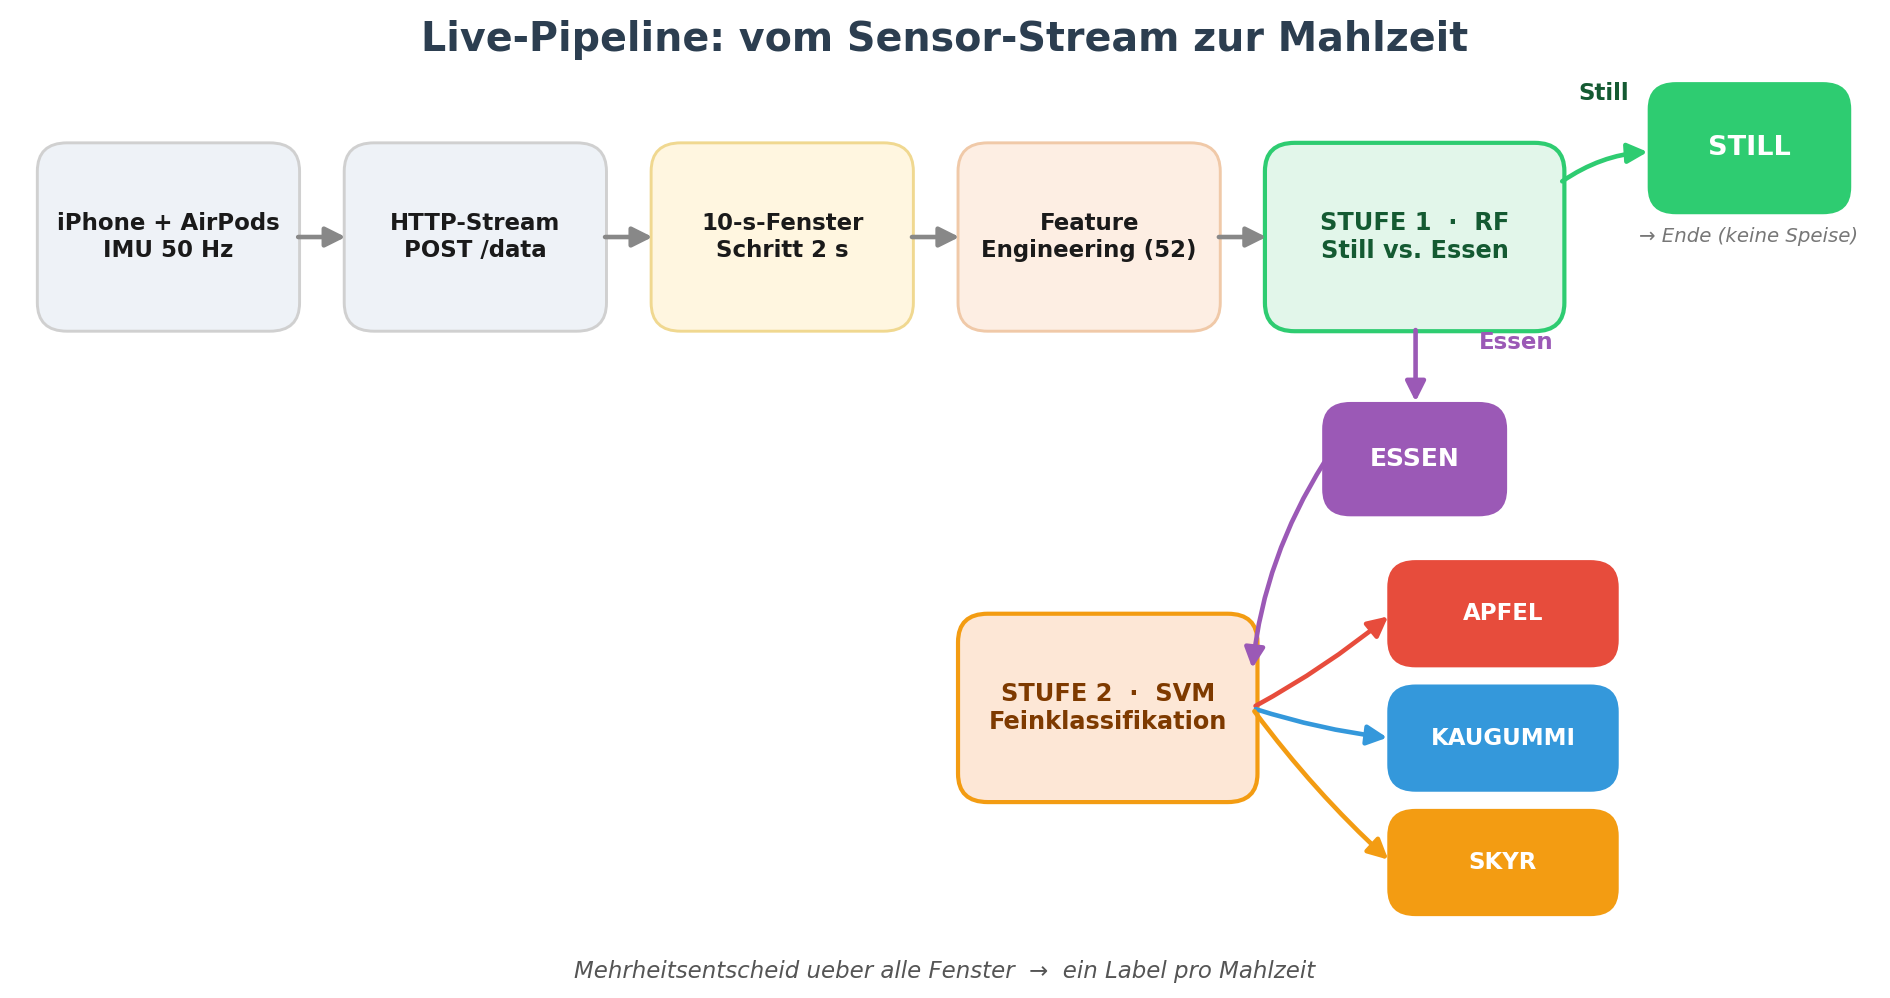
\includegraphics[width=.92\textwidth]{figures/final_pipeline_v2.png}
    \caption{Finale Pipeline vom Rohsignal über die Merkmalsextraktion zum hierarchischen
    Zwei-Stufen-Klassifikator.}
    \label{fig:pipe}
\end{figure}

Ein methodischer Schwerpunkt lag auf der Frage, welche Evaluationsstrategie ein ehrliches
Bild liefert. Bei fensterbasierten Daten liegt eine Falle in der klassischen
Leave-One-Out-Kreuzvalidierung pro Fenster: Fenster derselben Aufnahme sind einander sehr
ähnlich, sodass das Modell de facto auf Nachbarfenstern des Testfensters trainiert und die
gemessene Genauigkeit die reale Leistung systematisch überschätzt \citep[S.~3]{Saeb2017}.
Als ehrliche Metrik wurde deshalb durchgängig Leave-One-Session-Out verwendet, bei dem alle
Fenster einer Aufnahme gemeinsam als Testmenge ausgehalten werden. Das entspricht der in
der Aktivitätserkennung gebräuchlichen Leave-one-run-out-Strategie, mit der
personenspezifische Systeme bewertet werden, während Leave-one-person-out die
Generalisierung auf unbekannte Nutzer prüft \citep[S.~33:17]{Bulling2014}. Alle berichteten
Werte beziehen sich auf die ausgelieferte Konfiguration: Stufe~1 ist ein Random Forest mit
200 Bäumen auf 14 Merkmalen, arbeitet auf bewegungsbereinigten Fenstern und stuft eine
Vorhersage unterhalb einer Konfidenz von 0,75 auf Still zurück; Stufe~2 ist eine Support
Vector Machine ohne Movement Exclusion. Die Merkmalsauswahl der Stufe~2 wird innerhalb
jeder Falte neu bestimmt, sodass die Werte frei von Selektionsbias sind.

% ==================================================
\section{Ergebnisse}
% ==================================================

\subsection{Klassifikationsleistung}

Stufe~1 unterscheidet Stillsitzen und Essen mit einer Genauigkeit von 94,7\,\% bei einer
balancierten Genauigkeit von 94,5\,\%, gegenüber einer Mehrheitsbaseline von 76,6\,\%.
Stufe~2 erreicht über die drei Lebensmittel 88,7\,\% pro Fenster, mit klassenweisen
F1-Werten von 0,87 für Apfel, 0,84 für Kaugummi und 0,94 für Skyr. Auf Mahlzeitenebene, wo
jedes Fenster einer Mahlzeit abstimmt und das Mehrheitslabel gewinnt, steigt die
Genauigkeit auf 95,0\,\%, also 76 korrekt zugeordnete von 80 Mahlzeiten. Verkettet man
beide Stufen, liegt die Genauigkeit bei 87,5\,\% pro Fenster, bezogen auf 1319 Fenster, da
die 203 Fenster der generischen Sammelklasse keiner Zielklasse zugeordnet werden können,
und ebenfalls bei 95,0\,\% pro Mahlzeit; Stufe~1 verliert auf Mahlzeitenebene demnach
nichts. Abbildung~\ref{fig:cm} zeigt die zugehörigen Konfusionsmatrizen.

\begin{figure}[H]
    \centering
    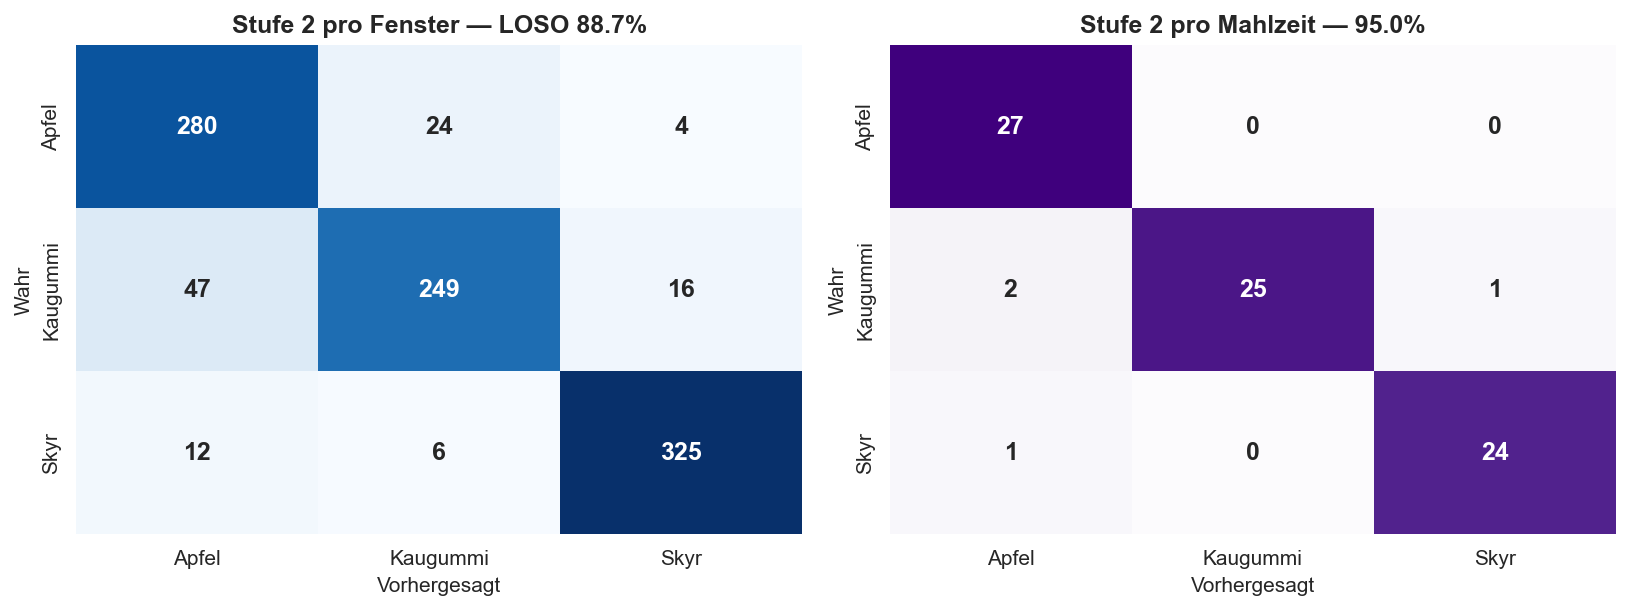
\includegraphics[width=.92\textwidth]{figures/final_stufe2.png}
    \caption{Konfusionsmatrizen der Stufe~2 unter LOSO: links pro Zehn-Sekunden-Fenster,
    rechts pro Mahlzeit nach Mehrheitsabstimmung.}
    \label{fig:cm}
\end{figure}

Die drei Werte messen dieselbe Modellleistung unter verschiedenen Bedingungen
(Abbildung~\ref{fig:bew}). Der Wert innerhalb der Aufnahmen von 93,8\,\% überschätzt, weil
das Modell benachbarte Fenster derselben Aufnahme kennt; der LOSO-Wert von 88,7\,\%
beschreibt die Übertragung auf eine unbekannte Aufnahme; die Aggregation pro Mahlzeit mit
95,0\,\% entspricht der Situation im tatsächlichen Einsatz, in dem nicht einzelne Fenster,
sondern das Ergebnis einer Mahlzeit zählt. Angesichts des kleinen Datensatzes ist auch der
LOSO-Wert vorsichtig zu interpretieren, da er die Generalisierung auf neue Aufnahmen
derselben Person beschreibt und nicht auf neue Personen. Der Wert pro Mahlzeit beruht zudem
auf nur 80 Mahlzeiten, sodass eine einzelne Fehlzuordnung ihn um mehr als einen
Prozentpunkt verschiebt.

\begin{figure}[H]
    \centering
    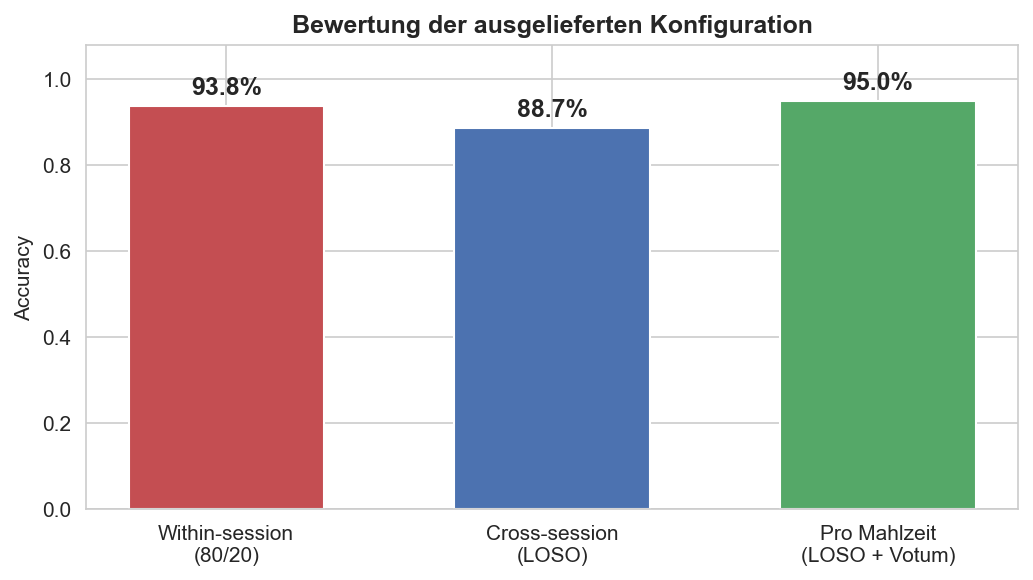
\includegraphics[width=.62\textwidth]{figures/final_bewertung.png}
    \caption{Dreistufige Bewertung: innerhalb der Aufnahmen (optimistisch),
    sessionübergreifend (realistisch) und pro Mahlzeit (Systemleistung).}
    \label{fig:bew}
\end{figure}

\subsection{Fehleranalyse und Klassendesign}

Die Fehleranalyse auf einem früheren Datenstand zeigte, dass sich fast alle Fehler auf eine
wechselseitige Verwechslung von Apfel und der generischen Klasse konzentrierten. Zwei
Ursachen wurden identifiziert. Erstens überlappen die realen Mahlzeiten der Sammelklasse im
Merkmalsraum mit den spezifischen Lebensmitteln; ein Experiment mit einer
Rückweisungsoption bestätigte dies, da die generischen Aufnahmen mit hoher Konfidenz falsch
klassifiziert werden. Es handelt sich also um ein Taxonomieproblem und nicht um ein
Konfidenzproblem, das ein Schwellwert lösen könnte. Zweitens entfernte die Movement
Exclusion die Crunch-Spitzen des Apfels; ohne sie stieg der Apfel-Recall auf dem damaligen
Datenstand von 62\,\% auf 78\,\%. Beide Befunde führten zur finalen Architekturentscheidung,
die generische Klasse aus Stufe~2 zu entfernen und ausschließlich in Stufe~1 zu belassen.
Allein diese Umstellung hob die Apfel-Präzision von 0,53 auf 0,76. Den größten
Genauigkeitsgewinn brachte damit das Klassendesign, nicht die Wahl des Modells.

Auf dem finalen Datensatz wurden zwei Stellschrauben gegeneinander geprüft. Die Movement
Exclusion macht in Stufe~2 kaum einen Unterschied, was die Entscheidung stützt, sie dort
abzuschalten. Die einmalig auf allen Daten bestimmte Merkmalsauswahl liefert dagegen
scheinbar bessere Werte als die faltweise bestimmte, nämlich 89,8 statt 88,7\,\% pro
Fenster und 98,8 statt 95,0\,\% pro Mahlzeit. Der Selektionsbias schlägt damit fast
ausschließlich auf die aggregierte Zahl durch, weshalb durchgängig die faltweisen Werte
berichtet werden.

Die Fehlerstruktur hat sich gegenüber den früheren Datenständen umgekehrt. Apfel wird nicht
mehr übersehen, sondern zu häufig vorhergesagt: Der Recall liegt bei 0,91, die Präzision
jedoch nur bei 0,83, weil zusätzlich 47 Kaugummi- und 12 Skyr-Fenster in der Apfel-Spalte
landen. Die Abschaltung der Movement Exclusion hat das Recall-Problem des Apfels also
behoben und dabei ein Präzisionsproblem erzeugt, das vor allem zulasten des Kaugummis geht.
Skyr ist mit einem F1-Wert von 0,94 die am besten trennbare Klasse; da alle drei Klassen
annähernd gleich viele Fenster umfassen, liegt das nicht an einem Datenübergewicht. Von den
109 falsch zugeordneten Fenstern entfallen 71 auf die Verwechslung von Apfel und Kaugummi.
Skyr unterscheidet sich im Signal also deutlich von beiden, was physikalisch naheliegt, da
es gelöffelt und kaum gekaut wird, während Apfel und Kaugummi echte Kaubewegungen erzeugen.

\subsection{Modellvergleich und Vergleich mit Deep Learning}

Zur Auswahl des Stufe-2-Modells wurden Random Forest, SVM, k-Nearest-Neighbors und ein
Multi-Layer Perceptron unter identischen Bedingungen auf 25-Sekunden-Fenstern verglichen. Das Ergebnis fiel eng aus:
Alle Modelle lagen innerhalb weniger Prozentpunkte, die SVM erzielte mit 94,1\,\% das beste
Ergebnis, knapp vor dem MLP mit 94,0\,\% und Random Forest sowie kNN mit je 93\,\%. Dieser
Vergleich wurde auf einem früheren Datenstand von 78 Aufnahmen und mit der optimistischen
fensterweisen Metrik durchgeführt und später nicht wiederholt; die absoluten Werte sind
daher als Zwischenstand zu lesen, der Vergleich der Modelle untereinander bleibt jedoch
gültig.

Um zu prüfen, ob ein Deep-Learning-Modell bessere Merkmale lernen könnte als die
handgefertigten, wurde ein 1D-Convolutional-Neural-Network direkt auf den rohen
Zehn-Sekunden-Fenstern mit sieben Kanälen trainiert, ergänzt um Datenaugmentierung. Für
einen fairen Vergleich wurden CNN und merkmalsbasierte SVM auf exakt denselben
sessionbasierten Splits evaluiert. Ohne Augmentierung erreichte das CNN 67,8\,\%, mit
Augmentierung 73,7\,\% und liegt damit 1,2 Prozentpunkte über der SVM mit 72,5\,\%. Ob
dieser Unterschied belastbar ist, lässt sich anhand der vorliegenden Daten nicht
entscheiden, da keine Signifikanzprüfung durchgeführt wurde; ein Vorteil des CNN lässt sich
daraus jedenfalls nicht ableiten. Alle drei Werte liegen unter den oben berichteten
Ergebnissen, weil dieser Vergleich noch auf dem Vier-Klassen-Problem einschließlich der
generischen Klasse beruht. Festhalten lässt sich damit, dass die handgefertigten Merkmale
den gelernten Repräsentationen hier nicht unterlegen sind, obwohl das CNN deutlich mehr
Rechenaufwand erfordert. Naheliegend, wenn auch im Rahmen dieses Projekts nicht geprüft,
ist die Vermutung, dass eher die Vielfalt der Daten als die Modellkapazität den
begrenzenden Faktor darstellt.

\subsection{Live-Anwendung}

Die Funktionsfähigkeit des Gesamtsystems wird durch eine Live-Webanwendung demonstriert.
Die AirPods streamen ihre Sensordaten per HTTP an einen lokalen Python-Server, der sie in
einen Ringpuffer von 20 Sekunden schreibt und daraus jeweils die letzten zehn Sekunden als
Klassifikationsfenster entnimmt. Alle zwei Sekunden wird klassifiziert und das Ergebnis an
ein Browser-Dashboard übertragen (Abbildung~\ref{fig:app}).

\begin{figure}[H]
    \centering
    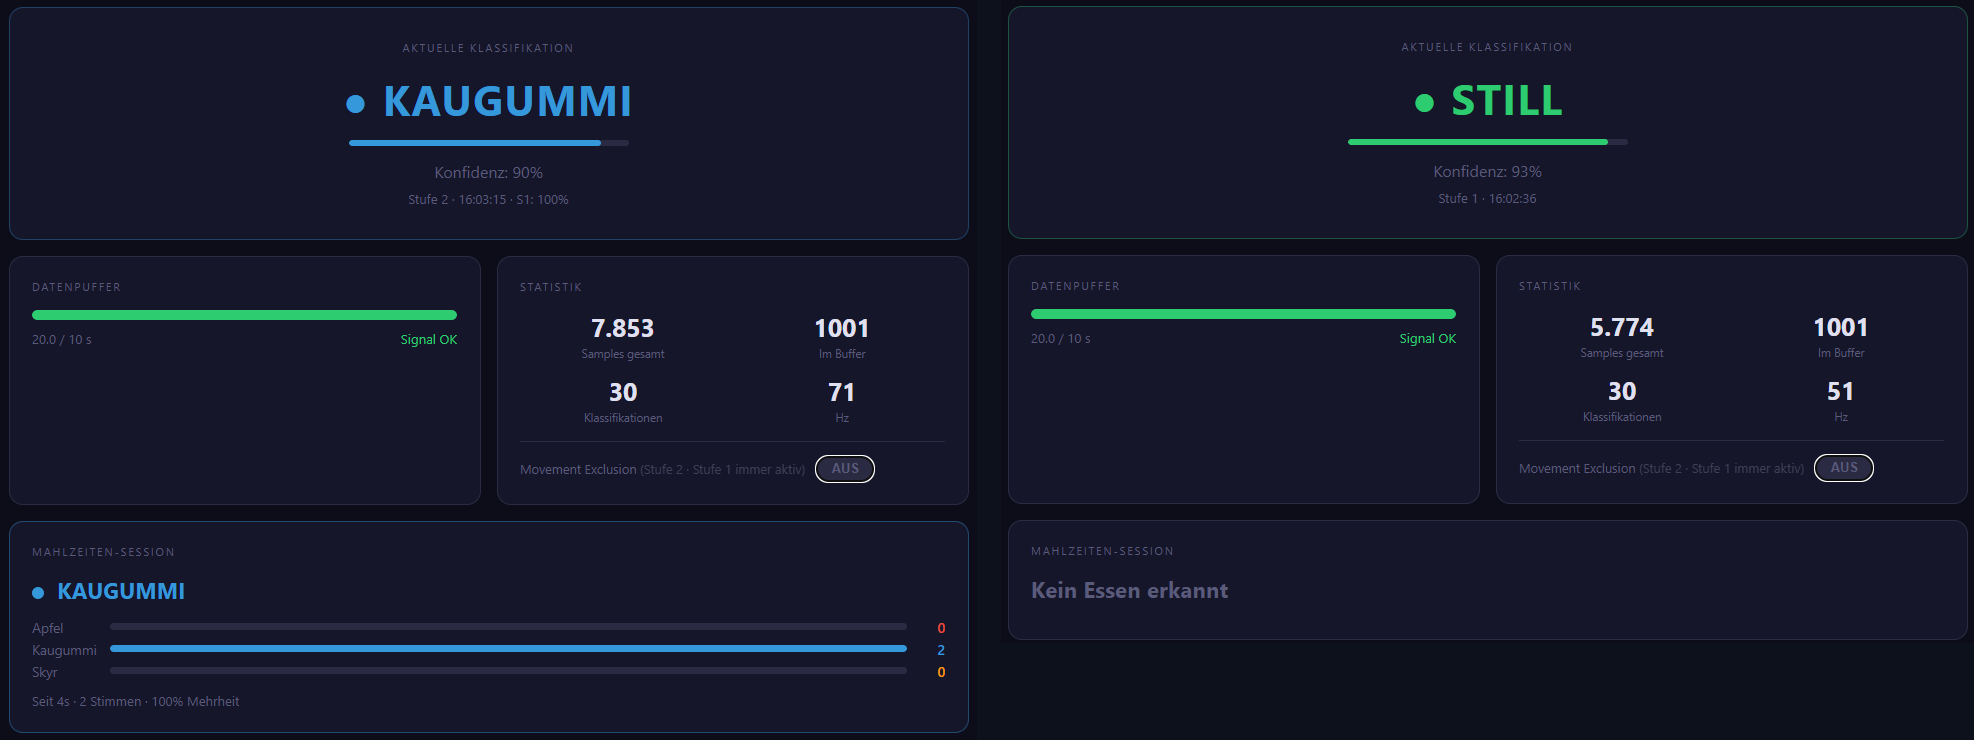
\includegraphics[width=.92\textwidth]{figures/app_live_kombi.png}
    \caption{Live-Ansicht der Anwendung in zwei Zuständen. Links wird während des
    Kaugummikauens in Stufe~2 klassifiziert, rechts erkennt bereits Stufe~1 Stillsitzen,
    sodass keine Lebensmittelklassifikation erfolgt.}
    \label{fig:app}
\end{figure}

Kernstück der Alltagstauglichkeit ist die zeitliche Aggregation pro Mahlzeit. Wann eine
Mahlzeit läuft, entscheidet ein einfacher Zustandsautomat: Fünf aufeinanderfolgende Fenster
mit der Vorhersage Essen eröffnen eine Mahlzeit, drei aufeinanderfolgende Still-Fenster
beenden sie. Diese Hysterese verhindert, dass einzelne Fehlklassifikationen eine Mahlzeit
auslösen oder abbrechen. Nur die Fenster innerhalb einer laufenden Mahlzeit geben eine
Stimme ab. Abbildung~\ref{fig:verlauf} zeigt beides im Betrieb.

\begin{figure}[H]
    \centering
    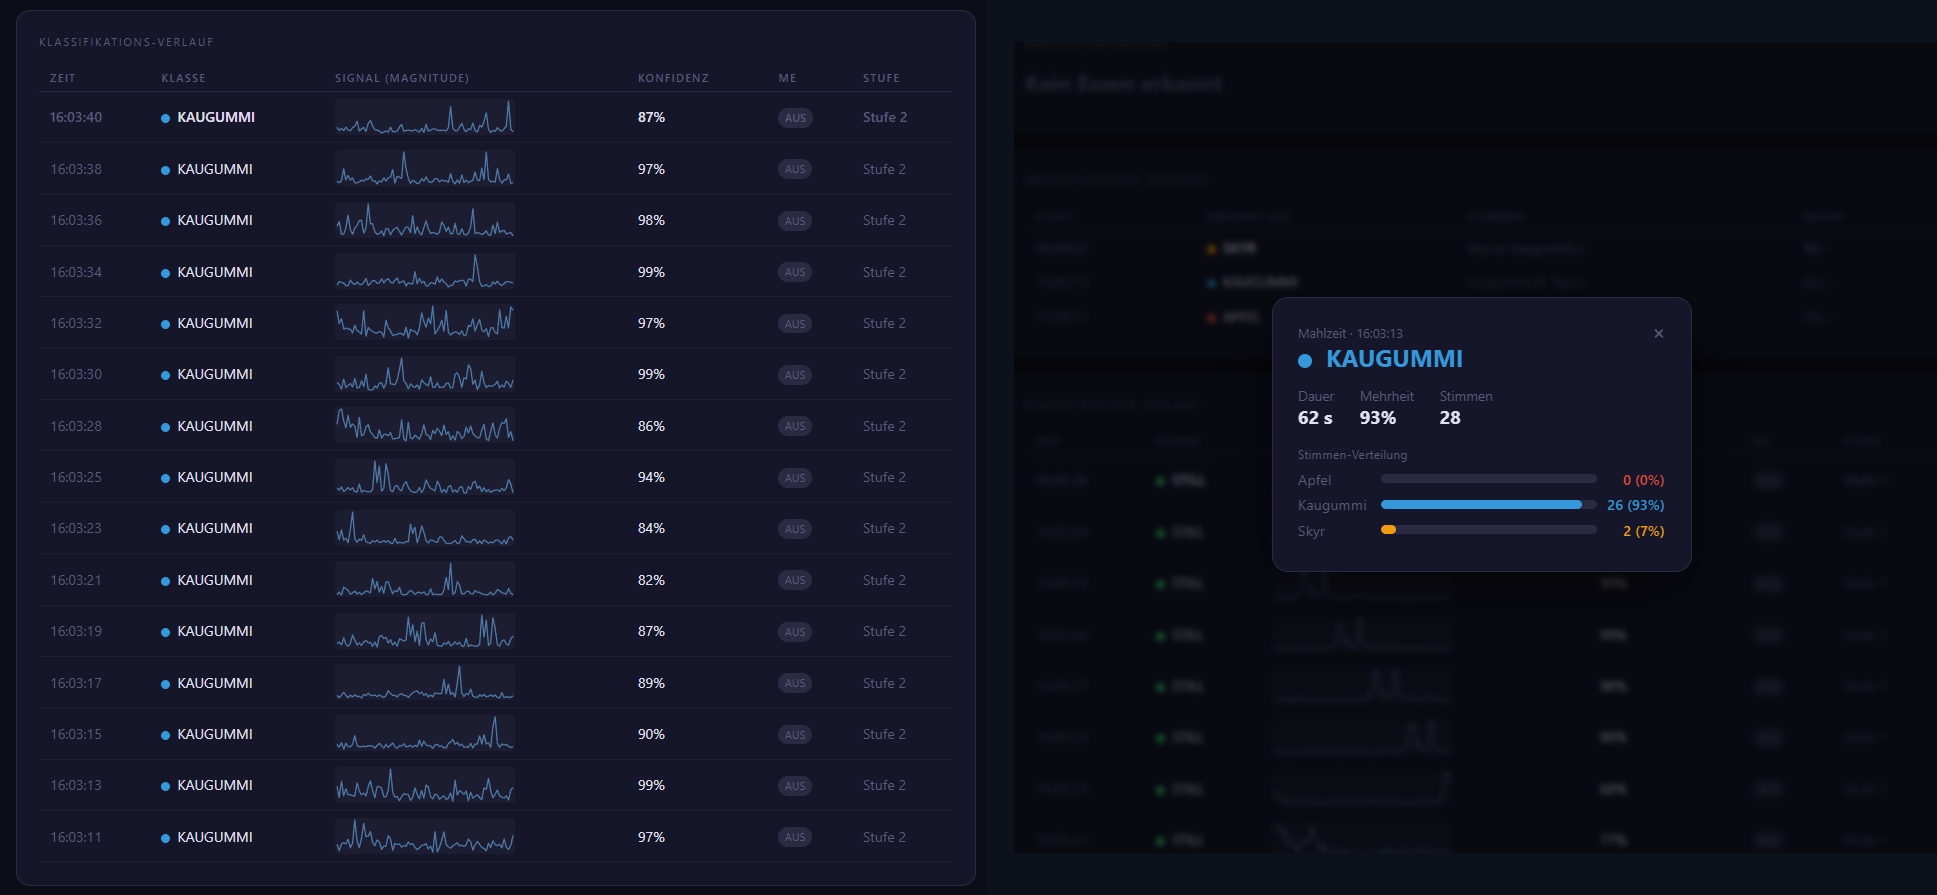
\includegraphics[width=\textwidth]{figures/app_verlauf_mahlzeit.png}
    \caption{Links der Klassifikationsverlauf, in dem alle zwei Sekunden ein Fenster
    ausgewertet wird; die Tabelle zeigt je Fenster das Magnitudensignal, die Konfidenz und
    die Stufe, in der die Entscheidung fiel. Rechts die Detailansicht einer abgeschlossenen
    Mahlzeit: Über 62 Sekunden wurden 28 Fenster klassifiziert, davon 26 als Kaugummi,
    woraus sich das Mehrheitslabel mit 93\,\% der Stimmen ergibt.}
    \label{fig:verlauf}
\end{figure}

Der Livebetrieb macht zwei Dinge sichtbar, die in den aggregierten Kennzahlen untergehen.
Erstens schwanken die Konfidenzen benachbarter Fenster derselben Mahlzeit erheblich,
im gezeigten Beispiel zwischen 82 und 99\,\%; einzelne Fenster sind also spürbar weniger
verlässlich als das Mehrheitslabel, was den Gewinn der Abstimmung anschaulich macht.
Zweitens traten Fehlklassifikationen einzelner Fenster tatsächlich auf, führten wegen der
Hysterese aber weder zu einem Fehlstart noch zu einem vorzeitigen Ende der Mahlzeit. Aus
dem Livetest stammt auch eine Korrektur am Modell: Die Konfidenzschwelle der Stufe~1 wurde
von 0,95 auf 0,75 abgesenkt, weil Apfelessen die strengere Schwelle häufig nicht passierte
und dadurch als Stillsitzen gewertet wurde. Ergänzend zeigt die Anwendung bei
abbrechendem Datenstrom einen expliziten Hinweis an, statt still das letzte Fenster zu
wiederholen.

Alle validierten Erkenntnisse der Modellierungsphase wurden übernommen, sodass sich die
oben berichteten Zahlen genau auf diese Konfiguration beziehen. Ein Unterschied bleibt: Die
Anwendung bestimmt die Merkmalsauswahl beim Start einmalig auf allen verfügbaren Daten,
während die Auswertung sie in jeder Falte neu berechnet.

% ==================================================
\section{Fazit und Ausblick}
% ==================================================

Die Forschungsfrage lässt sich für die untersuchte Einzelperson positiv beantworten:
Kaubewegungen, die über die IMU-Sensoren von AirPods Pro erfasst werden, erlauben sowohl
die Unterscheidung von Essen und Nicht-Essen als auch die Zuordnung zu einem von drei
bewusst sehr unterschiedlichen Lebensmitteln. Mit 88,7\,\% sessionübergreifender
Genauigkeit pro Fenster und 95,0\,\% pro Mahlzeit erreicht das System eine Leistung, die
ein passives Ernährungstracking auf unveränderter Consumer-Hardware zumindest als machbar
erscheinen lässt.

Rückblickend waren drei Entscheidungen ausschlaggebend, von denen keine die Wahl eines
besseren Modells betraf. Erstens die sessionübergreifende Evaluation, deren Einführung
aufdeckte, wie stark aufnahmespezifische Effekte die Ergebnisse verzerren, und die die
Arbeit auf die tatsächlichen Schwachstellen lenkte. Zweitens das Feature Engineering in
Kombination mit dem Entfernen sessionspezifischer Merkmale: Das wichtigste Einzelmerkmal
ist mit dem Jerk ein neu entwickeltes, und vier der sieben wichtigsten stammen aus der
Kaudynamik-Gruppe; das Aussortieren jener Merkmale, die vor allem die Kopfhaltung
kodieren, hob die sessionübergreifende Genauigkeit von 87,2 auf 88,7\,\%.
Drittens die Zerlegung in zwei Stufen samt dem daraus folgenden Klassendesign, die es
erlaubt, beide Stufen unterschiedlich zu behandeln; ein flaches Modell könnte die Movement
Exclusion nicht gleichzeitig nutzen und abschalten. Bemerkenswert ist schließlich, dass
sich die aus der Literatur abgeleitete Erwartung nicht bestätigte: Nicht der harte Apfel,
sondern das weiche Skyr erwies sich als die am besten trennbare Klasse. Eine mögliche
Erklärung ist, dass Skyr gelöffelt wird und sich dadurch deutlich von den beiden gekauten
Klassen abhebt; das bleibt allerdings eine Hypothese.

Die zentrale Limitation bleibt die Datenbasis, da sämtliche 103 Aufnahmen von einer Person
stammen. Alle Kennzahlen beschreiben daher die Generalisierung auf neue Aufnahmen derselben
Person; ob das Modell auf andere Personen mit anderer Anatomie und anderen Kaugewohnheiten
übertragbar ist, konnte nicht geprüft werden. Hinzu kommt, dass die Merkmalsauswahl nicht
stabil ist, da je nach Trainingsdaten zwischen 14 und 48 der 52 Merkmale gewählt werden,
was auf eine begrenzte Robustheit des Verfahrens bei dieser Datenmenge hindeutet. Die
Einzelarbeit wirkte sich vor allem auf die Datenerhebung aus, und erschwerend kam hinzu,
dass sich mit jeder Erweiterung des Datensatzes sämtliche Kennzahlen verschoben, sodass
laufend festzuhalten war, welches Ergebnis auf welchem Datenstand entstanden ist.

Der nächstliegende Schritt ist daher eine Erhebung mit fünf bis zehn Probanden, evaluiert
mit Leave-One-Subject-Out. Zu erwarten wäre, dass die Genauigkeit zunächst spürbar sinkt,
da Kiefergeometrie, Sitz der AirPods und Kaugewohnheiten variieren. Aufschlussreich wäre
vor allem, welche Merkmale diesen Wechsel überstehen; die Vermutung liegt nahe, dass
rhythmusbasierte Größen stabiler bleiben als amplitudenabhängige, weil sie beschreiben, wie
gekaut wird, und nicht wie stark. Sollte sich das bestätigen, wäre eine personenspezifische
Kalibrierung über eine kurze Referenzaufnahme eine naheliegende Erweiterung. Auf
Systemebene wäre die Schätzung der Kauanzahl pro Mahlzeit reizvoll, wie sie IMChew
verfolgt, da sich daraus eine Gesundheitsmetrik ableiten ließe; die nötigen Bausteine sind
in der Pipeline bereits vorhanden. Perspektivisch könnte ein solcher Ansatz an Bedeutung
gewinnen, wenn Geräte am Kopf weiter verbreitet sind. Für Anwendungen zum
Ernährungstracking läge der Gewinn vor allem in der Bedienung: Statt dass Nutzer jede
Mahlzeit von sich aus eintragen, könnte die Anwendung bei erkannter Essaktivität nachfragen
und ein Lebensmittel vorschlagen. Der Grundgedanke ist nicht neu, denn \citet{Bell2020}
nennen zwei Studien, in denen das Gerät bei erkannter Essbewegung unmittelbar nachfragt
\citep[S.~9]{Bell2020}; neu wäre der Vorschlag des konkreten Lebensmittels, der die Eingabe
auf eine Bestätigung reduziert. Sämtliche genannten Punkte sind Vorschläge und wurden im
Rahmen dieses Projekts nicht überprüft.

\medskip
\bibliography{references.bib}

\newpage
% ==================================================
\section*{Anhang}
% ==================================================

\textbf{Repository.} Der vollständige Code, sämtliche Rohaufnahmen, die Notebooks und die
Live-Anwendung liegen unter
\url{https://github.com/karstensjonah-design/ML4CS-group-ChewML}. Die Struktur umfasst
\texttt{data/raw/} mit einem ZIP-Archiv pro Aufnahme, \texttt{notebooks/} mit 14 Analyse-
und Experimentier-Notebooks (02--15), \texttt{ml\_httpstreaming/} mit der Live-Anwendung,
\texttt{reports/} mit den wöchentlichen Projektberichten, den Abbildungen und dem
Quelltext dieses Papers sowie
\texttt{sources/} mit der verwendeten Literatur.

\medskip
\noindent\textbf{Beiträge der Teammitglieder.} Das Projekt wurde nach einem Gruppenwechsel
in der fünften Semesterwoche als Einzelarbeit durchgeführt. Datenerhebung, Vorverarbeitung,
Merkmalsentwicklung, Modellierung, Evaluation, Live-Anwendung sowie sämtliche Berichte,
Präsentationen und dieses Paper stammen vollständig von Jonah Karstens.

\medskip
\noindent\textbf{Verwendete Werkzeuge.} Modelle, Kreuzvalidierung und Merkmalsselektion
wurden mit scikit-learn umgesetzt \citep{Pedregosa2011}, Signalverarbeitung und
Merkmalsberechnung mit NumPy, pandas und SciPy, das 1D-CNN mit PyTorch. Die vollständige
Liste mit Versionsangaben steht in der Datei \texttt{requirements.txt} im Repository. Für
Code und Auswertung wurden KI-gestützte Werkzeuge eingesetzt.

\end{document}
